\chapterimage{Intro/Intro_Figures/ArtisticView2.jpg} % Chapter heading image
%Einstein Telescope artists impression copyright Nikhef
%\section{Introduction}
\chapter{Introduction}
\label{chap:Intro}

\subsection[Prologue]{Prologue}
\label{Prologue}
The upgrade from the first to the second generation of gravitational wave detectors (GWDs) has brought a wealth of detections and enabled the observation of a variety of events leading to great scientific results and insights into astrophysical processes. The sensitivity achieved with the advanced detectors produces gravitational wave candidates of binary black holes almost weekly, but the signal-to-noise ratio (SNR) of all previous and the vast majority of expected detections is too low for precise astronomical investigations of the GW sources and many highly interesting sources (e.g. neutron star infusions or supernovae) are still too rare in the current detection range. \par
Long before the first gravitational wave detection the GW community started investigating a new (third) generation of detectors. In particular, the European Commission supported the European GW community to perform a conceptual design study within the Seventh Framework Programme (FP7-Capacities).\par 
With a considerably improved sensitivity, new detectors of the third-generation will open the era of routine precision GW astronomy and with the Einstein Telescope (ET) project Europe will lead this scientific revolution. The \bf{detection} of gravitational waves had been the goal of the advanced, the current generation. Now the focus is shifting to astrophysical \bf{observations}, which is why we call the Einstein Telescope an GW \bf{observatory} instead of a GW \bf{detector}.\par
To realise a third-generation GW observatory with a significantly enhanced sensitivity (we defined a target of a factor of ten improvement in sensitivity for ET with respect to the advanced detector design sensitivity over a wide frequency range), limitations of the technologies adopted in the advanced interferometers which would limit the next generation machines must be overcome. The Einstein Telescope will use some such new technologies, listed in this report.\par
The first and main target of this document is the definition of  the requirements and of the main characteristics of the site hosting ET, the design of the key elements of the research infrastructure, an evaluation of the costs and of the timeline of its implementation. To understand the importance and the need of the site and infrastructures in the ET design it is worth to recall the history of the current GW detector infrastructures, shown in Fig.~\ref{Fig:InfraEvolution}.

The next generation of gravitational wave observatories will need new infrastructures for several reasons:
\begin{itemize}
    \item The first and second generation of GWDs are using the same infrastructure which by now is more than 25 years old and will have reached an age of 40 years by the anticipated start of operation of the Einstein Telescope. The aging would require a complete overhaul of the infrastructure with associated long down-times.
    \item The sensitivity that can be achieved in the existing infrastructures by implementing new technologies will be limited by the constraints of the site and infrastructure (arm length, local seismic noise, absence of cryogenic apparatus, vacuum pipe size\,\ldots).
    \item Upgrades to the existing infrastructures can be done in a staged way, allowing for a more or less continuous series of observation runs, with only moderately long interruptions. Radical upgrades of the existing detectors (e.g. going to cryogenic operation at a different wavelength) would require down-times on the order of more than five year. 
\end{itemize} 
In order to realise a third-generation GW observatory like ET, an infrastructure hosting several detectors that evolve for many decades is crucial.

explain how the science goals are correlated with and lead to the design of the observatory

adapt old intro chapter and update it


\clearpage

\subsection{Scientific targets of the ET observatory}
\subsubsection{Fundamental physics}
\label{ScienceCase:FundamentalPhysics}
Astronomical sources of gravitational waves are essentially
systems where gravity is extremely strong, and are often
characterized by relativistic bulk motion of massive objects.
The emitted radiation carries an uncorrupted signature of the
nature of the space-time geometry, and is thus an invaluable
tool to understand the behaviour of matter and geometry in
extreme conditions of density, temperature, magnetic fields
and relativistic motion. Here are some examples of how GW
observations can impact fundamental physics.

In Einstein's theory, gravitational radiation travels at the speed 
of light and has two polarization states. In alternative theories 
of gravity one or both of these properties might not hold, owing 
to the presence of massive gravitons, or a scalar field mediating 
gravity in addition to the tensor field. Current experimental
tests of gravity, as well those afforded by the data from the
Hulse-Taylor binary, are consistent with both Einstein's theory
and one of its alternatives called the Brans-Dicke theory.
Gravitational wave detectors will bring these theories
vis-a-vis observations that could decisively rule out one
or the other.

According to Einstein's gravity the space-time in the vicinity
of black holes is described by a unique geometry called the
Kerr solution. Observation of the radiation from the infall
of stellar-mass black holes into intermediate-mass black holes
will make it possible to test such uniqueness theorems. X-ray
astronomy has provided firm indirect evidence that intense
sources of X-rays may well host a black hole. An unambiguous
signature of the black hole geometry, however, could eventually
be provided by the detection of black hole quasi-normal modes:
gravitational radiation with characteristic frequencies and decay
times that depend only on the mass and spin angular momentum of the black hole.
Failure to detect such radiation from, for example, a newly
formed black hole would mean that gravity is more exotic than
we currently believe,
%(e.g., gravitational collapse might lead to entities called naked singularities)
and might reveal new phases of matter at extremely high densities.

The most attractive versions of string theory require a ten- or
eleven-dimensional space-time, far above those that we perceive.
In certain phenomenological models at the interface of string
theory and cosmology, what we perceive as a four-dimensional
Universe could be one part, or ``brane'', within a higher
dimensional ``bulk'' Universe. The extra spatial dimensions may
be compact and sub-millimetre-scale,
%(so-called ``Large Extra Dimensions'')
or even macroscopically large, if their geometry has
properties known as ``warping''. The key feature of brane-world
theories is that gravitational interactions, and in particular
gravitational waves, propagate in the bulk, while other interactions
are restricted to the brane, which partly explains why gravity is
so weak. 
%Brane world models predict a specific signature in the spectrum of gravitational waves. 
% [DON"T KNOW HOW WE CAN STAND BEHIND THIS SENTENCE, ITS 
% NOT SUPPORTED BY THE SCIENCE CASE]
Third-generation detectors offer 
the exciting possibility of observing radiation from the bulk and 
thereby exploring whether the Universe has large extra dimensions.
% SOME STUFF ABOUT HOW TO TEST STRING THEORY \& BRANES
% OR COMMENTS ON NEW PHYSICS IN GENERAL IN RELATION TO
% STOCHASTIC?



\FloatBarrier
\subsubsection{Relativistic Astrophysics}
Astronomy has revealed a Universe full of diverse and exotic phenomena that remain enigmas decades after their discovery.
Supernovae are the end-states of stellar evolution, resulting in gravitational collapse followed by a huge explosion of the formerly infalling matter.
Gamma-ray bursts are intense sources of gamma radiation that last only a few seconds to minutes yet emit more energy than a star does in its entire lifetime.
Radio pulsars are compact objects as massive as the Sun but only about 10\,km in size, and the regularity of their radio pulses and occasional glitches in that regularity have remained  puzzles for a long time after their discovery three decades ago.
Transient radio sources thousands of light years away are associated with magnetic fields so strong that the emitted radiation could break down terrestrial radio stations.

The source in question in each case is believed to be couched in dense environs and strong gravitational fields and, therefore, a potential source of gravitational radiation. For example, gamma-ray bursts could be produced by colliding neutron stars which are electromagnetically invisible for most of their lives but are very powerful emitters of GWs. Transient radio sources could be the result of quakes in neutron stars with concomitant emission of GWs.
Observing such `multi-messengers' (sources that are strong emitters of both EM and GW radiation) will help understand phenomena that have remained puzzles for decades.

The centre of every galaxy is believed to host a compact object a million to a billion times as massive as our Sun, a powerful emitter of optical, radio and other radiation.
What is the nature of this object? How and when did it form?
Did it form from small 100-solar-mass seeds and then grow by accreting gas and other compact objects? What is its relation to the size of the galaxy as a whole.
These are some of the questions which a model of the formation of structure in the Universe must answer.  
While electromagnetic observations  have provided valuable data, ET can explore the population of stellar mass and intermediate mass black holes as a function  of redshift and shed light on black hole demographics, their 
mass distribution and growth.
ET will also be sensitive to a population of sources at very high redshifts, helping us study cosmological evolution of sources, the history of star formation and its dependence on the matter content of the Universe, and the development of large-scale structure in the Universe. 
\FloatBarrier
\subsubsection{Cosmology}
The twentieth century was the golden age of cosmology. With the advent of radio and microwave astronomy it was possible to finally address key questions about the origin of the Universe.  
The cosmic microwave background (CMB) is a relic radiation from the hot Big Bang that is believed to have been the initial condition for primordial nucleosynthesis.
Since the early Universe was very dense, this radiation was in thermal equilibrium with matter for about 380,000 years after the Big Bang and cannot directly reveal the conditions in the very early phases of the Universe's history. 
The most direct way of observing the primeval Universe is via the gravitational window with a network of two or more detectors. 
From fairly general assumptions one can predict the production of a stochastic background of GWs in the early Universe, which travel to us unscathed as a consequence of their weak coupling to matter.

The most amazing aspect of the Universe is that only about 4\% of its energy density appears in the form of visible matter, the rest being dark matter and dark energy. 
In order to understand the behaviour of these `dark' contents it is necessary to have a standard candle---a population of sources whose distance from Earth can be inferred from their luminosity. 
Compact binaries are an astronomer's ideal standard candle. 
By measuring the signature of the gravitational radiation they emit, it is possible to infer their intrinsic parameters (e.g.\ the masses and spins of the component objects) and accurately deduce their luminosity distance. In fact, compact binaries
eliminate the need to build a cosmic distance ladder---the process by which standard candles at different distances are calibrated in astronomy since there is no source that is suitable at all distances.

The synergy of multi-messenger astronomy is nowhere more apparent than in the use of standard sirens of gravity to test the concordance model of cosmology.  ET might detectseveral hundred compact  binary coalescence events each year in coincidence with short-hard gamma-ray bursts, provided, of course, the two are related.  While gravitational observations would provide an unambiguous measure of the luminosity distance, the host galaxy of the GRB could be used to measure the redshift. By fitting the observed population to a cosmological model, it will be possible to measure the Hubble parameter, dark matter and dark energy densities, as well as the dark energy equation-of-state parameter.

The early history of the Universe may have witnessed several phase transitions as the temperature decreased through the energy scales of a Grand Unified Theory (GUT) and electroweak symmetry-breaking, and eventually to the current state in which we see four different fundamental interactions. During some phase transitions, cosmic strings form as one-dimensional topological defects at the boundaries of different phases. Vibrations of these strings at the speed of light can sometimes form a kink that emits a burst of gravitational radiation. The spectrum of such radiation has a unique signature that can help us detect cosmic strings and measure their properties, and thus provide a glimpse of the Universe as it underwent phase transitions.

Perhaps the most exciting discovery of the new window willbe none of the above. If astronomical history is any example, gravitational astronomy should unveil phenomena and sources never imagined in the wildest theories---a possibility of any new observational tool.


\FloatBarrier
\newpage
\subsection{Layout of the detector}
%\emph{Authors: M.Punturo, H. Lueck} 

\begin{wrapfigure}{r}{0.6\textwidth}
\vskip -0.4cm
	\centering
	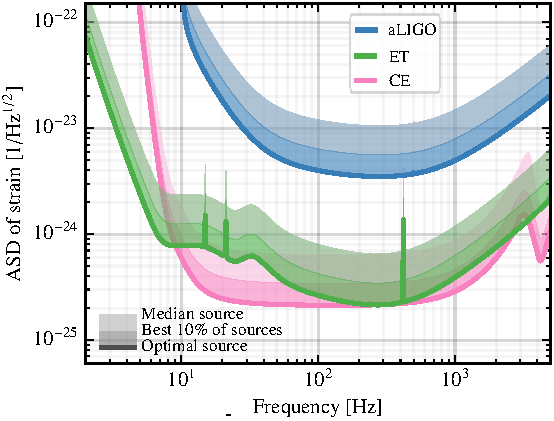
\includegraphics[width=0.6\textwidth]{Intro/Intro_Figures/noises_percentiles-Voyager(1).pdf}
	\caption{Design sensitivities of the advanced and the third generation gravitational wave detectors. The various colour shades represent different sets of source locations and orientations.}
	\label{fig:GW_sens_evolution}
\end{wrapfigure}
The sensitivity of gravitational wave detectors improved considerably from 
the bar detectors through the first generation of interferometric detectors to the currently operating \textit{advanced}, 2nd generation. The sensitivities of the 2nd and 3rd generation are shown in figure~\ref{fig:GW_sens_evolution}. 
In order to achieve the scientific goals stated above, the sensitivity in comparison to the second generation of gravitational wave detectors must be improved by about an order of magnitude over the entire detection frequency band ranging from 10\,Hz to about 10\,kHz. Frequent and precise observation of low-frequency sources, e.g.\ intermediate mass black holes, requires an extension of the detection range towards lower frequencies. \\
The sensitivity goal for the Einstein Telescope, as shown in figure~\ref{fig:GW_sens_evolution}, was driven by the need to get frequent high Signal to Noise Ratio (SNR) events for routine gravitational wave astronomy. The high-frequency sensitivity is given by the maximum power feasible, the mid-frequency range is governed by thermal noises and the low-frequency range by either thermal or seismic noises.\\
\subsubsection{Size, shape and layout}
The conceptual design of a project of this financial scale (see table~\ref{Fig:TotalCostTable}) must be based on well proven and experimentally tested techniques. To achieve the sensitivity that the Einstein Telescope project aims for, on the other hand, it will be necessary to exploit all state-of-the-art technologies and drive them to their physical limits.
\begin{wrapfigure}{r}{0.4\textwidth}
%\begin{figure}{H}
	\centering
		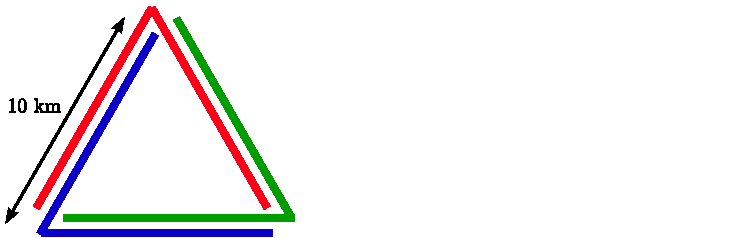
\includegraphics[width=0.3\textwidth]{Intro/Intro_Figures/NestedDetectors.pdf}
	\caption{Three nested detectors in a triangular arrangement will 
	form the final Einstein Telescope geometry.}
	\label{fig:NestedDetectors}
\end{wrapfigure}
This sensitivity can only be reached by significantly increasing the size of the 
detector beyond the size of currently available instruments (i.e.\ 3\,km for advanced Virgo 
and 4\,km for advanced LIGO) and going to an underground location, where the seismic 
noise is lower than at the surface. Only by increasing the arm length to 10\,km 
can the influence of unavoidable displacement noises be lowered to a tolerable 
level.\\
In its final construction stage the Einstein Telescope will consist of three nested
detectors, which will be arranged in a triangular pattern as shown in 
figure\,~\ref{fig:NestedDetectors}. 
In contrast to the traditional L-shaped geometry of the first and second generations 
of gravitational wave detectors this arrangement is equally sensitive for both 
polarisations of the gravitational wave. Additionally it shows a more isotropic 
antenna pattern compared to the L-shaped detectors, as shown in 
figure\,~\ref{fig:response}. The overall frequency range covered will reach from 
a few Hertz to about 10\,kHz.

Each individual detector in turn will comprise two interferometers, one 
specialised for detecting low-frequency gravitational waves and the other one 
for the high-frequency part. The sensitivity goal for each interferometer is shown 
in figure\,\ref{fig:ET_sensitivity}. %\\
Each individual interferometer has a classical dual-recycled Michelson topology 
with arm cavities. This is a mature technique, well tested in laboratory 
experiments, and currently being set up for the second-generation detectors, 
Advanced LIGO and Advanced Virgo. More elaborate topologies like Sagnac 
interferometers or optical bars using Quantum Non-Demolition (QND) techniques 
do not promise significant advantages and have not yet reached the level of 
maturity required for a project of this scale.\\

\subsubsection{Quantum Noise} 
In order to achieve a sufficient sensitivity at high frequencies the light power in 
the arms of the high-frequency interferometer needs to be increased to the 
megawatt range. Thermal noise considerations on the other hand require cryogenic 
optics to reach the sensitivity goal at low frequencies. 

\begin{wrapfigure}{r}{0.6\textwidth}
%\begin{figure}{H}
	\centering
		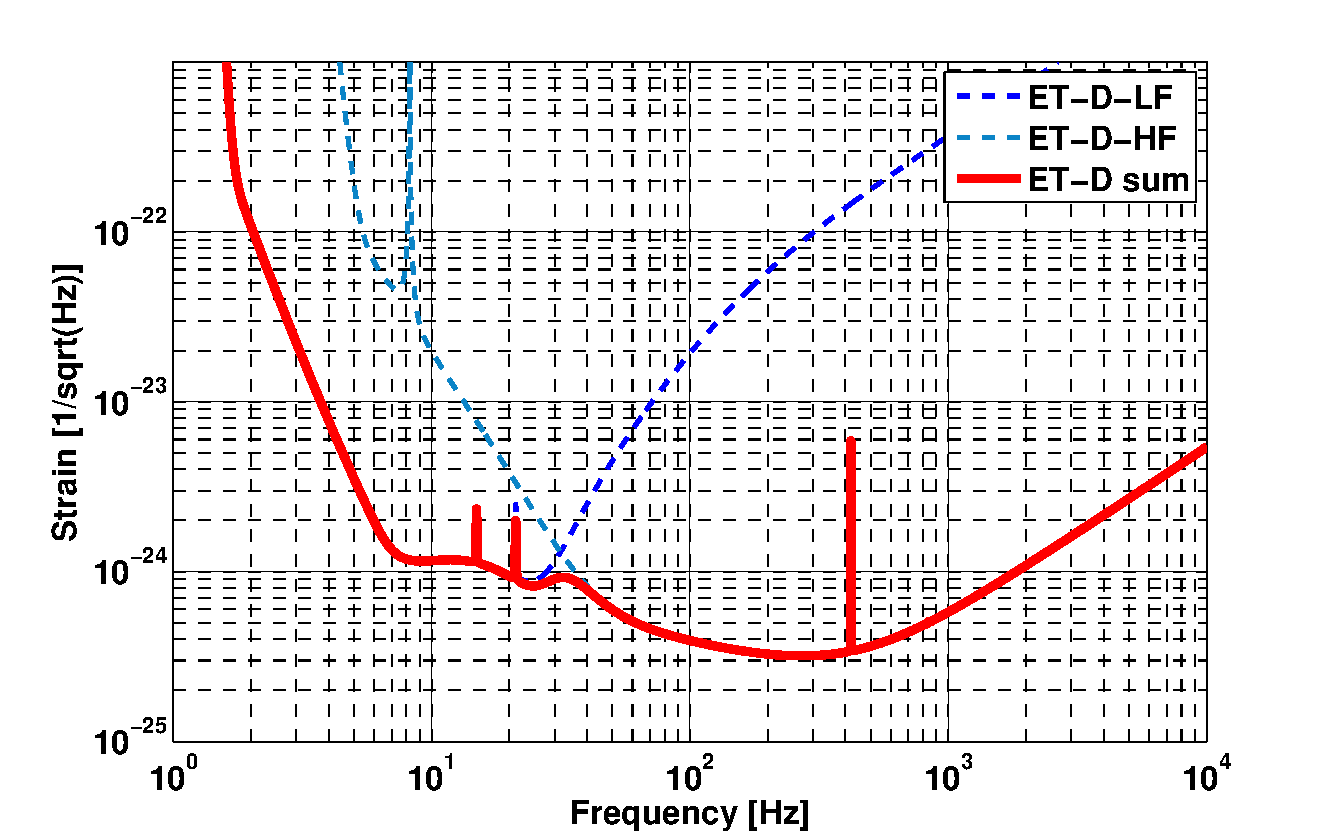
\includegraphics[width=0.6\textwidth]{Intro/Intro_Figures/ET_D_spectrum.pdf}
	\caption{Sensitivity of the Einstein Telescope in the `xylophone' configuration. 
	The sensitivity of the low-frequency cryogenic interferometer is shown in the 
	dashed dark blue curve and the one of the high-frequency room temperature 
	one in a dashed blue-green tone. The sum of both is given by the solid bright red curve.}
	\label{fig:ET_sensitivity}
\end{wrapfigure}

Operating cryogenic optics at a level of several megawatt of light power presents 
a serious technological challenge which is extremely hard to master. Even for 
the best mirrors that state-of-the-art coating technology can produce, the 
residual absorption of only about one ppm leads to an absorbed power of 
several Watt at a circulating light power level in the megawatt range. The resulting 
thickness of the suspension fibres, which would be needed to remove the heat, 
would spoil the performance of the ultra low loss suspension. The Einstein 
Telescope will therefore be realised in what we call a `xylophone' arrangement, 
where each single detector is split into two interferometers, leading to sensitivities 
as shown in figure~\ref{fig:ET_sensitivity}. The one dedicated for detecting 
high-frequency gravitational waves in the range from about 30\,Hz to 10\,kHz 
will be operated at room temperature, use fused silica optics with a diameter of 
about 60\,cm and a mass of about 200 kg each, have a light power of about 3\,MW 
in the interferometer arms, and run with broadband tuned signal recycling. The 
cryogenic, low-frequency one, operated at a temperature of 10\,K and aimed at the 
frequency range from 1.5\,Hz to 30\,Hz, will use detuned signal recycling, have a 
light power of 18\,kW 
in the interferometer arms, and silicon mirrors with a diameter of about 40\,cm and 
a mass of about 200\,kg. The cryogenic optics will either be made of sapphire or, 
more likely, of silicon. The dimensions will partly be determined by the maximum 
available bulk material size and otherwise be comparable to the room temperature 
ones. A summary of the main parameters for the high and low temperature 
interferometers is given in table~\ref{tab:summary14}.\\
The high mirror mass will not only keep radiation pressure effects low but also 
allow larger sized beam spots on the mirror surfaces for lowering thermal noise 
effects. This split detector arrangement also offers an elegant solution for the 
challenge that radiation pressure noise and shot noise scale in opposite ways with 
light power and cannot individually be optimised in a single interferometer. In an 
interferometer using classical states of light the so-called Standard Quantum 
Limit (SQL) determines the lower limit for the quantum noise. For each frequency 
there is a different optimal compromise between shot noise and radiation pressure 
noise, meaning that in a single interferometer the SQL cannot be reached for all 
frequencies simultaneously. 
 
\begin{wrapfigure}{r}{0.35\textwidth}
%\begin{figure}{H}
	\centering
		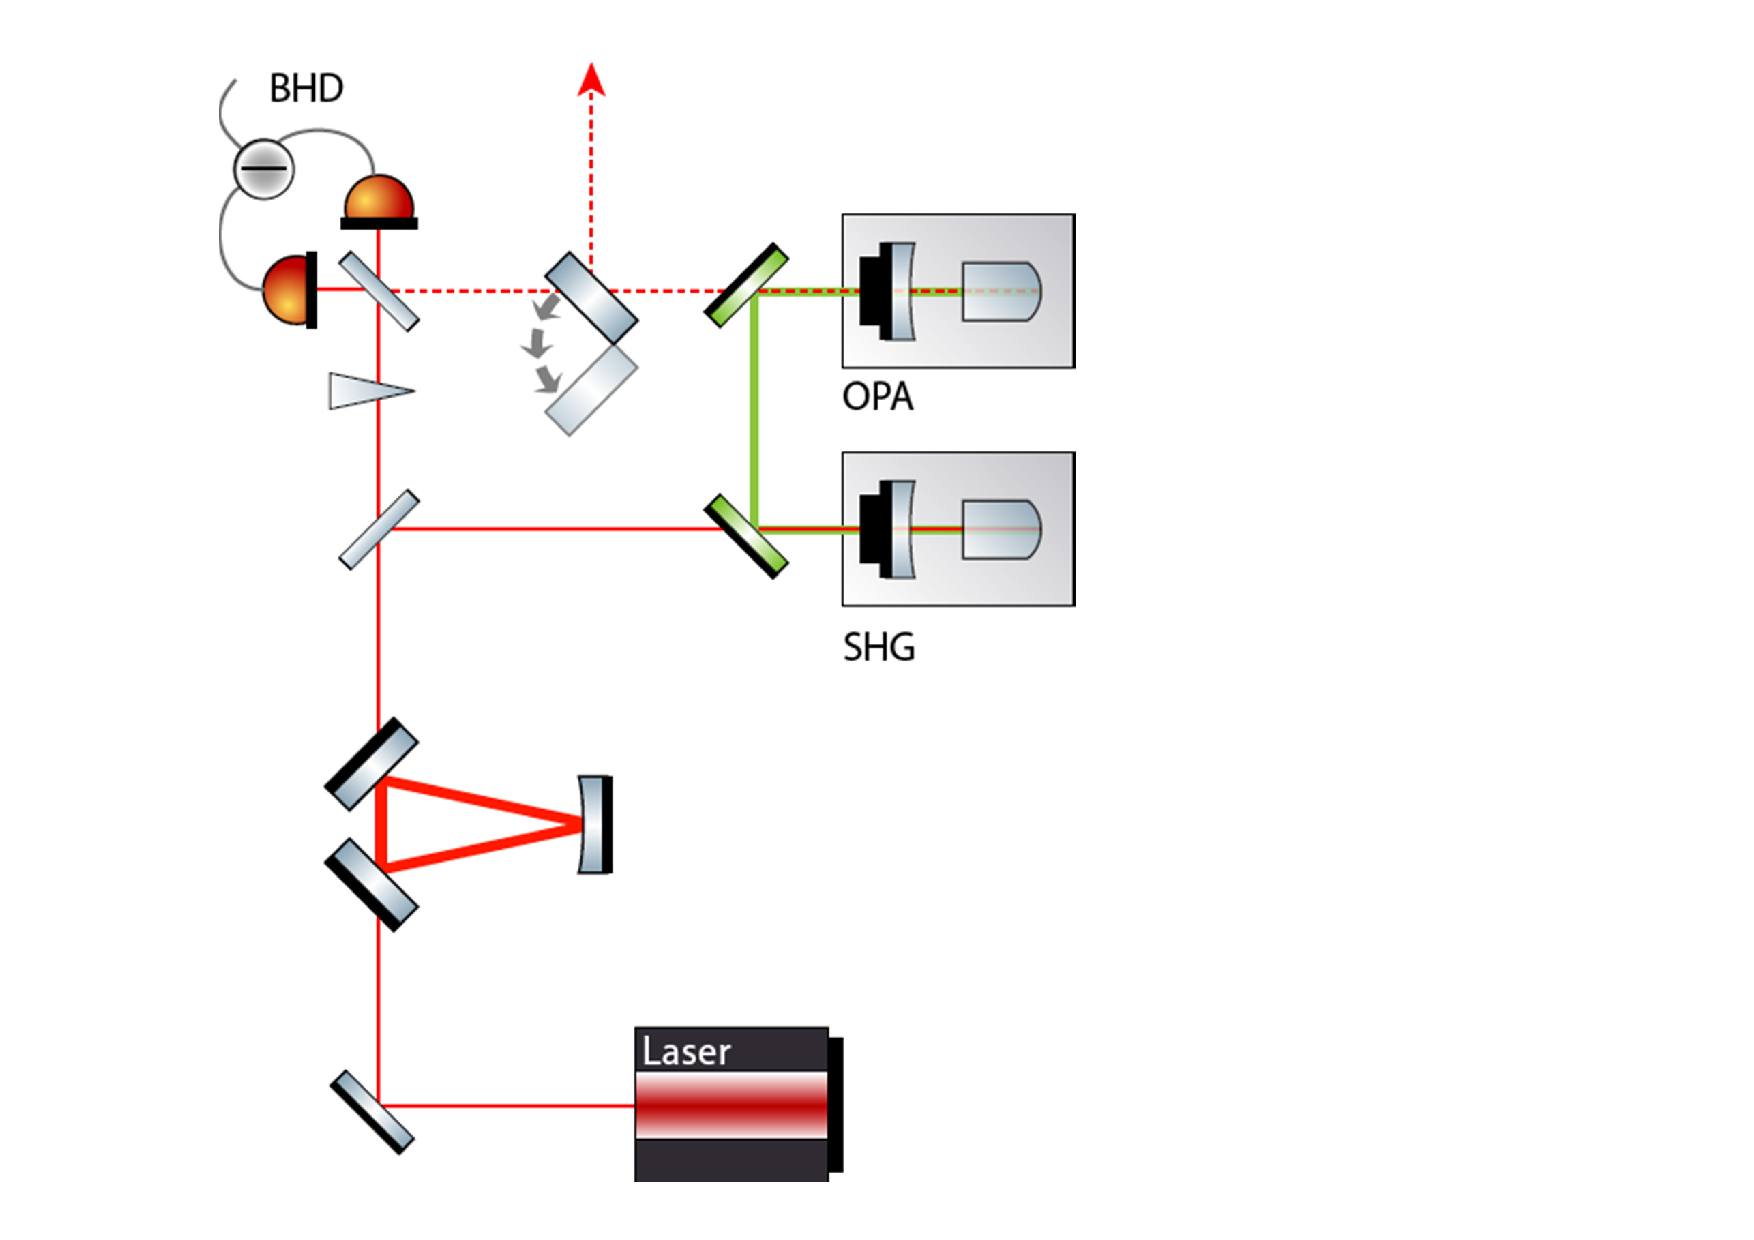
\includegraphics[width=0.35\textwidth]{Intro/Intro_Figures/SqzGenIntro.pdf}
	\caption{Scheme for generating squeezed light. For details see section~\ref{subsec:SQZforGWD}}
	\label{fig:SqzGenIntro}
\end{wrapfigure} 

It can only be overcome if non-classical light with correlations between the phase 
and the amplitude quadratures is used, so-called squeezed light. In the shot noise 
dominated frequency range squeezed light is used, which shows lower phase 
fluctuations at the cost of the amplitude fluctuations in comparison to classical 
laser light in the interferometer arms. In the low-frequency, radiation pressure 
dominated range the fluctuations need to be lowered in the amplitude quadrature. 
This goal can be achieved by reflecting squeezed light off a filter cavity (see 
figure~\ref{Fig:opt_lay_over}). 

The usage of squeezed light is currently tested in the existing gravitational wave 
detectors and is foreseen as an add-on to the second generation. Squeezing 
levels over the full observation band width of up to 10\,dB, and stable long-term 
operation and best squeezing values of almost 13\,dB have been demonstrated~\cite{Eberle2010}. 
For the Einstein Telescope we assume 15\,dB initial squeezing 
level at the squeezing source and an effective squeezing level of 10\,dB to be 
available (equivalent in shot noise reduction to a laser power increase of a factor
of 10). 

The squeezing level, and with it the sensitivity improvement that can be reached, 
depends on the optical losses in the squeezer, the filtering optics, the interferometer, 
and all optical devices on the way to the photodetector, including the photodetector 
efficiency itself. Optical losses easily add vacuum fluctuations to the squeezed quadrature 
and hence reconvert squeezed light into classical light. It will therefore be essential 
to keep the optical losses as low as possible. Optical losses of 75\,ppm per round 
trip are currently achievable with state-of-the-art techniques and are used as a 
conservative estimate for the filter cavities.

\subsubsection{Thermal Noise}
\begin{wrapfigure}{r}{0.65\textwidth}
\vskip -0.6cm
%\begin{figure}{H}
	\centering
		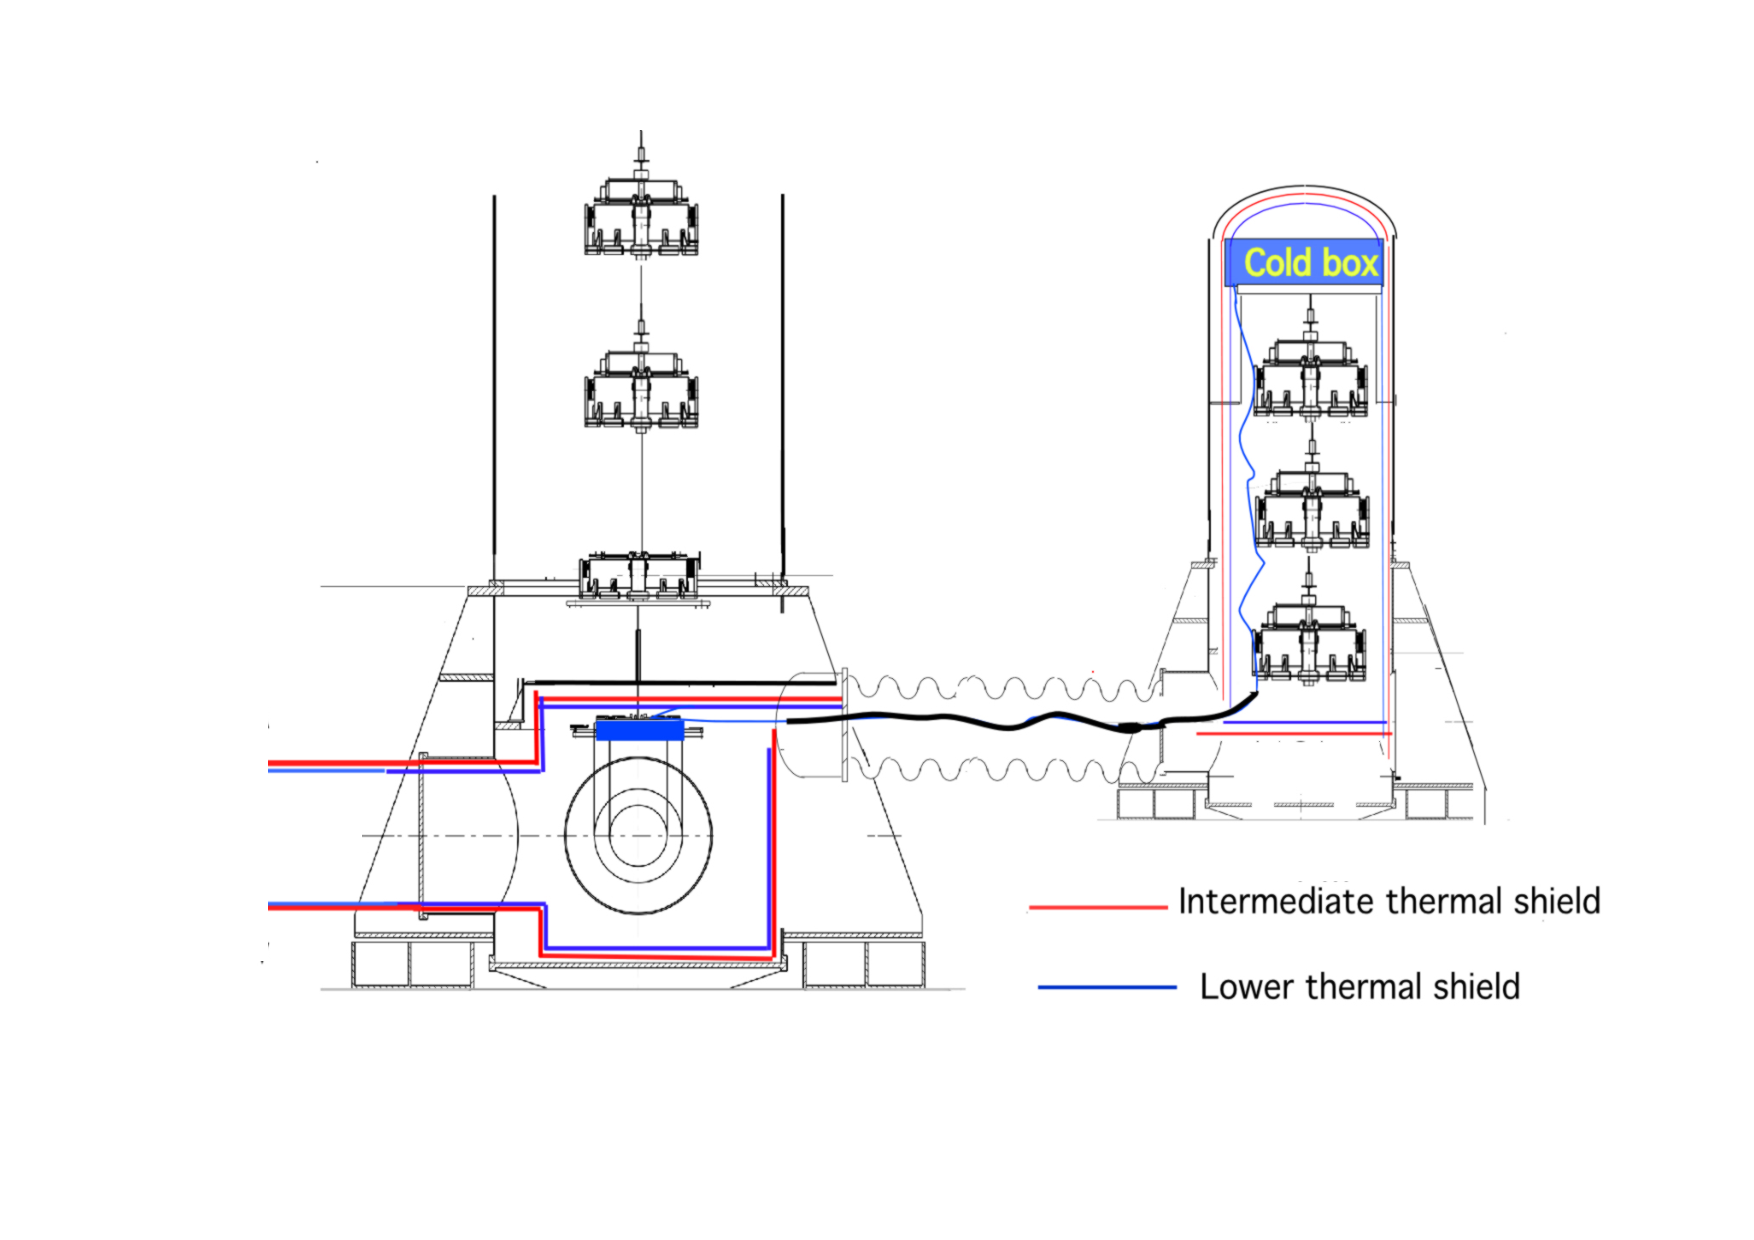
\includegraphics[width=0.6\textwidth]{./Intro/Intro_Figures/ET_main-cryostat.pdf}
	\caption{Scheme for cooling the mirrors. For details see section~\ref{cryo}}
\vskip -0.1cm
\end{wrapfigure} 

Reaching the sensitivity goal at low frequencies requires a significant reduction 
of thermal noises compared to the first and second generations of gravitational-wave 
detectors, which can be achieved by operating the mirrors at cryogenic temperatures 
as low as 10\,K.  

Cryogenic operation is also used in the Japanese gravitational wave detector KAGRA. At these low temperatures fused silica has a low mechanical quality factor and becomes unusable. Silicon and sapphire show 
excellent low-temperature behaviour (see section~\ref{sec:app}) and are good 
candidates for cryogenic gravitational wave detectors. Its availability in large 
quantities and good purity through the semiconductor industry makes silicon a 
promising candidate for the Einstein Telescope cryogenic optics. Some quantities 
such as the temperature dependence of the refractive index at low temperatures 
and the residual optical absorption in ultra pure silicon, although assumed to be 
good enough for use in ET, are currently not known and need to be 
investigated in R\&D activities.

Removing the heat generated by laser light being absorbed at the mirror surfaces 
without introducing excess vibration levels poses another technical challenge. As 
thermal radiation does not provide sufficient coupling at cryogenic temperatures 
this heat removal has to be done by thermal conduction of the suspension fibres. 
The resulting requirement for the thickness of the silicon suspension fibres needs 
to be balanced against good seismic isolation properties of thin fibres. The vibration 
level of cryo coolers, which could be placed close to the optics, threatens the 
low-frequency sensitivity (see section~\ref{sec:cryocoolers}). R\&D in active and 
passive vibration suppression is still required to sufficiently cut the remaining noise 
level down for use in the Einstein Telescope. Cryo fluids, like superfluid Helium\,II, 
which are cooled down at a remote location above ground, are available as a 
seismically more quiet alternative (see section~\ref{sec:Helium_II}). The final operating 
temperature for ET remains to be fixed in a technical design 
phase. The cooling capabilities foreseen so far will allow mirror temperatures 
as low as 10\,K.

\subsubsection{Seismic Isolation}

\begin{wrapfigure}{r}{0.4\textwidth}
\vskip -0.4cm
%\begin{figure}{H}
	\centering
		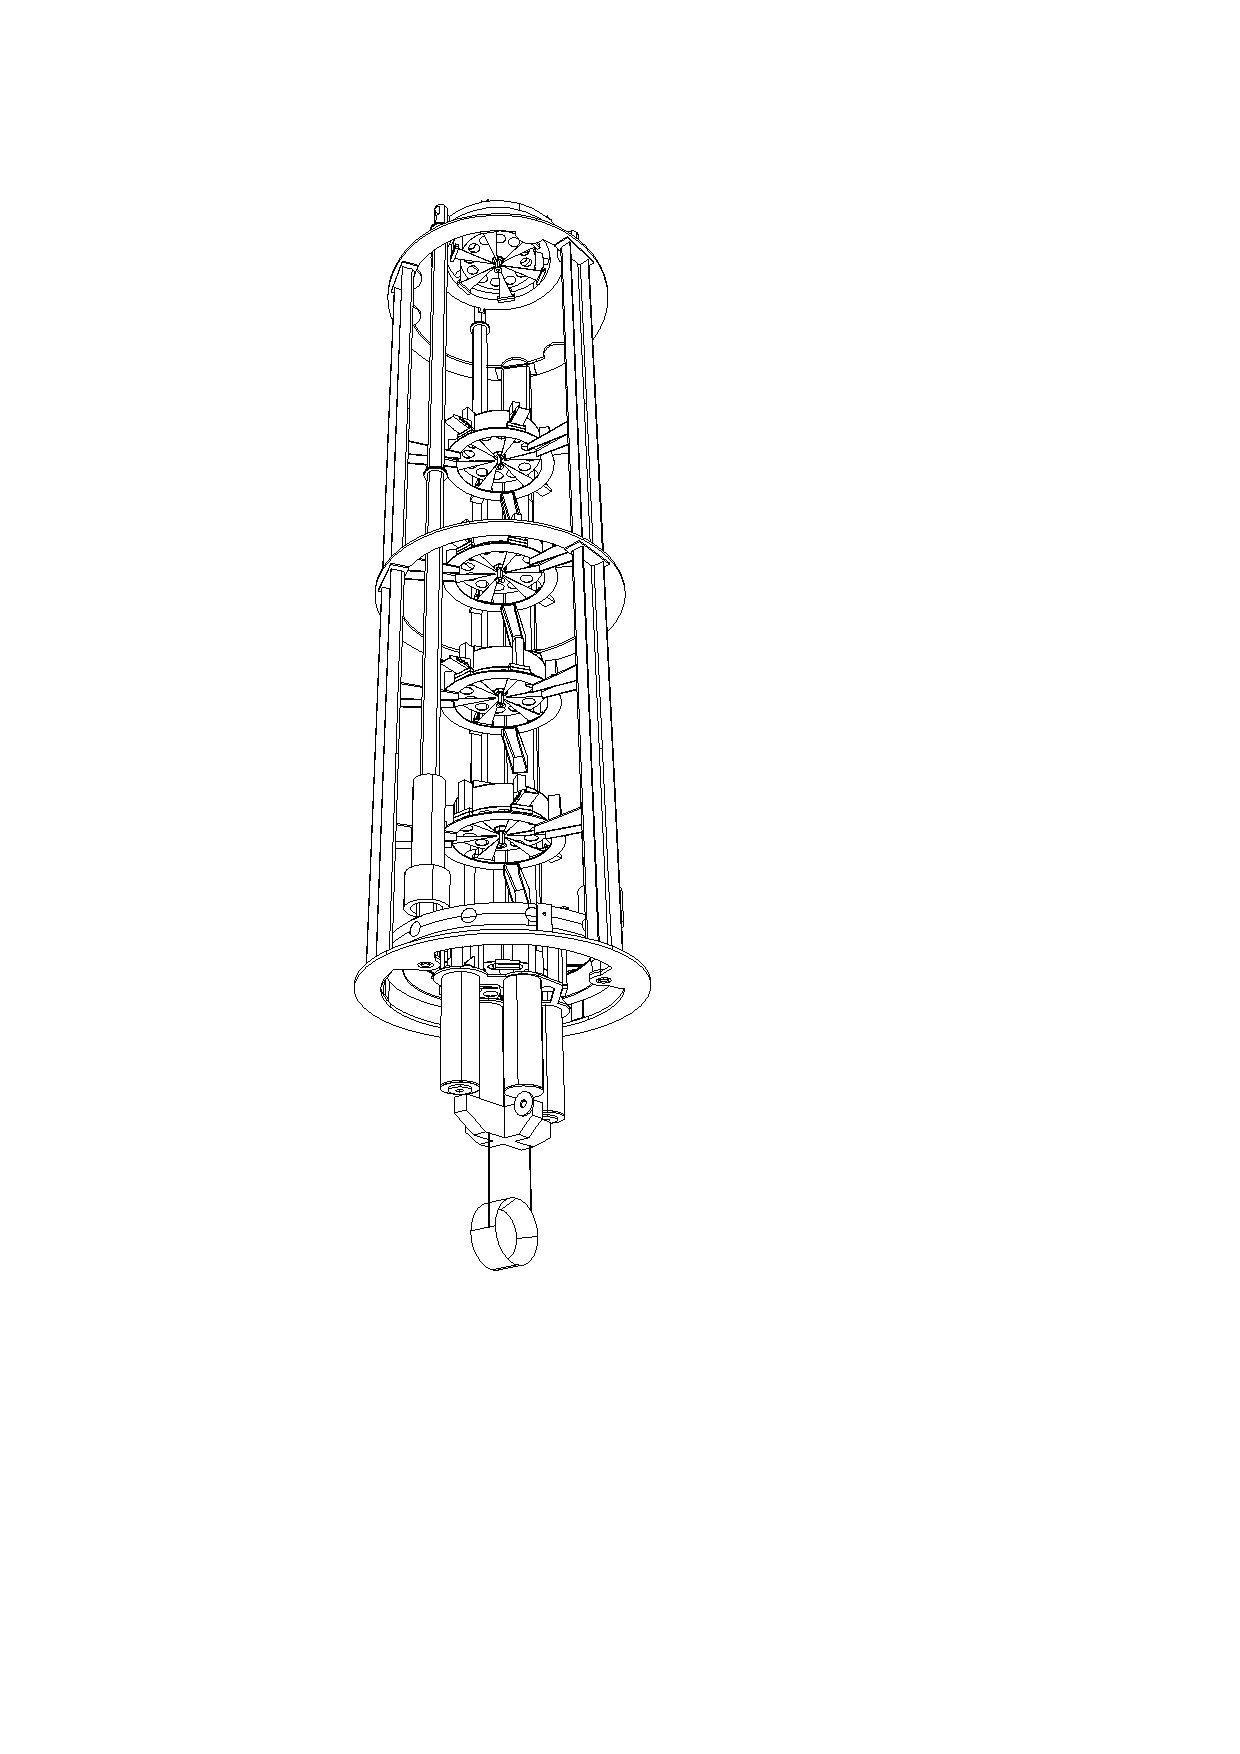
\includegraphics[width=0.18\textwidth]{./Intro/Intro_Figures/VirgoSA.pdf}
\vskip 0.3cm
	\caption{Schematic view of the Virgo Superattenuator. See also section~\ref{sec:suspension_systems}}
\vskip -0.6cm
\end{wrapfigure} 

The main optics for the Einstein telescope need to be very well isolated against 
seismic ground motion. For the second generation of gravitational wave detectors 
both active and passive isolation strategies are being pursued. In the advanced 
LIGO detectors a two stage system actively isolates a platform from ground 
motion, from which the main optics are suspended by quadruple pendulums. The 
passive strategy employed at the Virgo detector demonstrated an excellent 
performance over the full frequency range (see figure \ref{FigSusp5}) and is foreseen 
as the reference solution for the Einstein telescope. The horizontal isolation is 
achieved with a six-stage pendulum system, whereas for the vertical degree of 
freedom cantilever springs  are used. The pendulum suspension system itself is 
supported by a platform resting on an inverted pendulum, which provides 
additional horizontal seismic isolation (see figure~\ref{SAfig1}). All mechanical 
resonances of the whole structure are actively damped to avoid resonant 
mechanical amplification of ground motion. The overall height of the suspension 
system is about 17\,m, requiring correspondingly tall vacuum chambers and caverns.

\subsubsection{Newtonian gravity gradient noise}
Newtonian gravitational interactions between the optics and the surrounding soil 
provide a direct coupling mechanism of ground motion to the interferometer test 
masses (see also section~\ref{NewtonianNoise}). As the resulting, so-called 
gravity gradient noise cannot be shielded from the mirrors, a location has to be 
found where this seismic motion is minimal and the surrounding soil as 
homogeneous as possible. This goal can be achieved in an underground location 
in a seismically quiet region. Preliminary measurements show that a depth of 100 to 
200\,m in a remote location with low population density provides sufficiently low 
seismic motion. The potential of measuring the ambient seismic motion, feeding 
it into a gravity gradient noise model, and then subtracting the predicted effect 
from the interferometer output signal has been investigated. Initial results are 
promising, and are interesting also for the second generation of gravitational 
wave detectors, but investigations need to be continued in an R\&D programme 
(see section~\ref{subsub:AmbientNNsubtraction}).

\subsubsection{Vacuum}
The space between the mirrors in the interferometer arms has to be evacuated 
to very low residual partial gas pressures to keep the apparent length changes 
caused by fluctuations of the refractive index sufficiently low. The tolerable 
maximum pressure is on the order of $10^{-8}$\,Pa (see paragraph~\ref{average pressure}).
 
Some technical parameters will remain ``to be defined'' in this design study 
document. At this stage of the conceptual design these parameters are not 
important and will be worked out in a future technical design phase.

\subsubsection{\label{Noisebudget}Noise budget}

\begin{wrapfigure}{r}{0.60\textwidth}
  \begin{center}
\vskip -0.3cm
    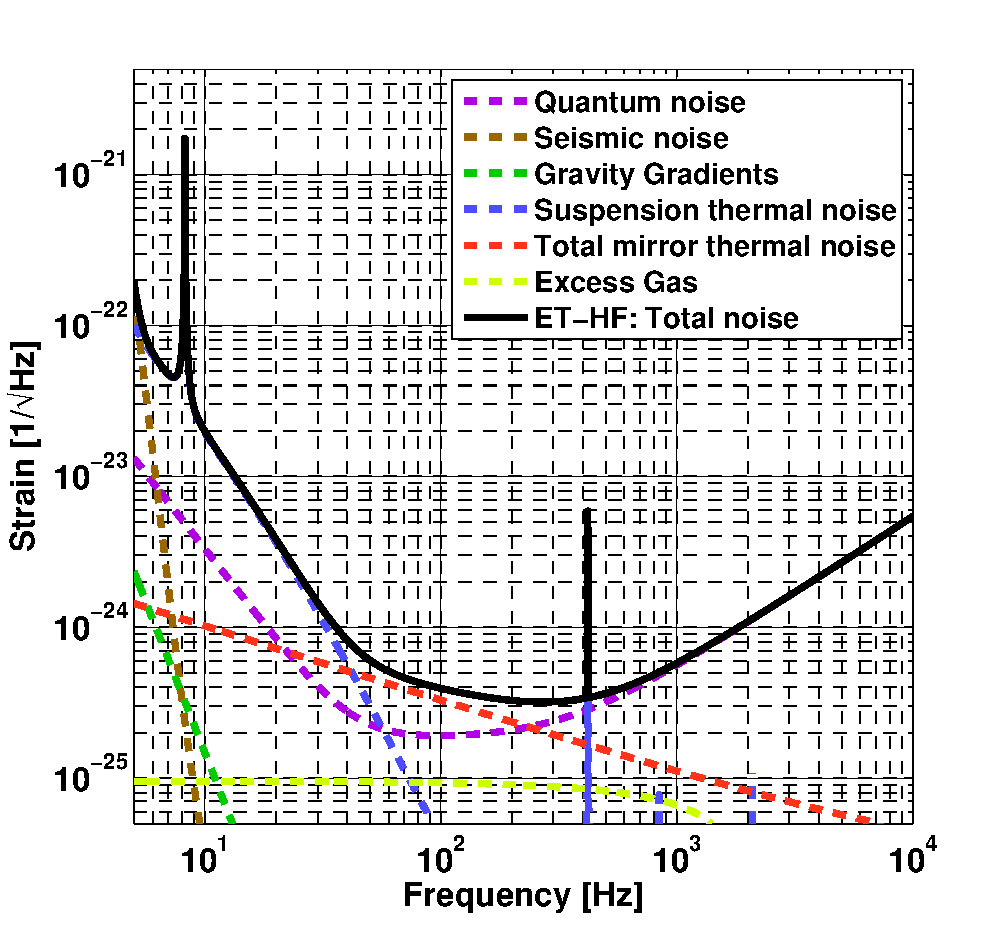
\includegraphics[width=0.45\textwidth]{Intro/Intro_Figures/ETD_HF3.pdf}
%      \end{center}
%  \end{wrapfigure}
%  
% \begin{wrapfigure}{r}{0.6\textwidth}
%  \begin{center}
\vskip 0.4cm
    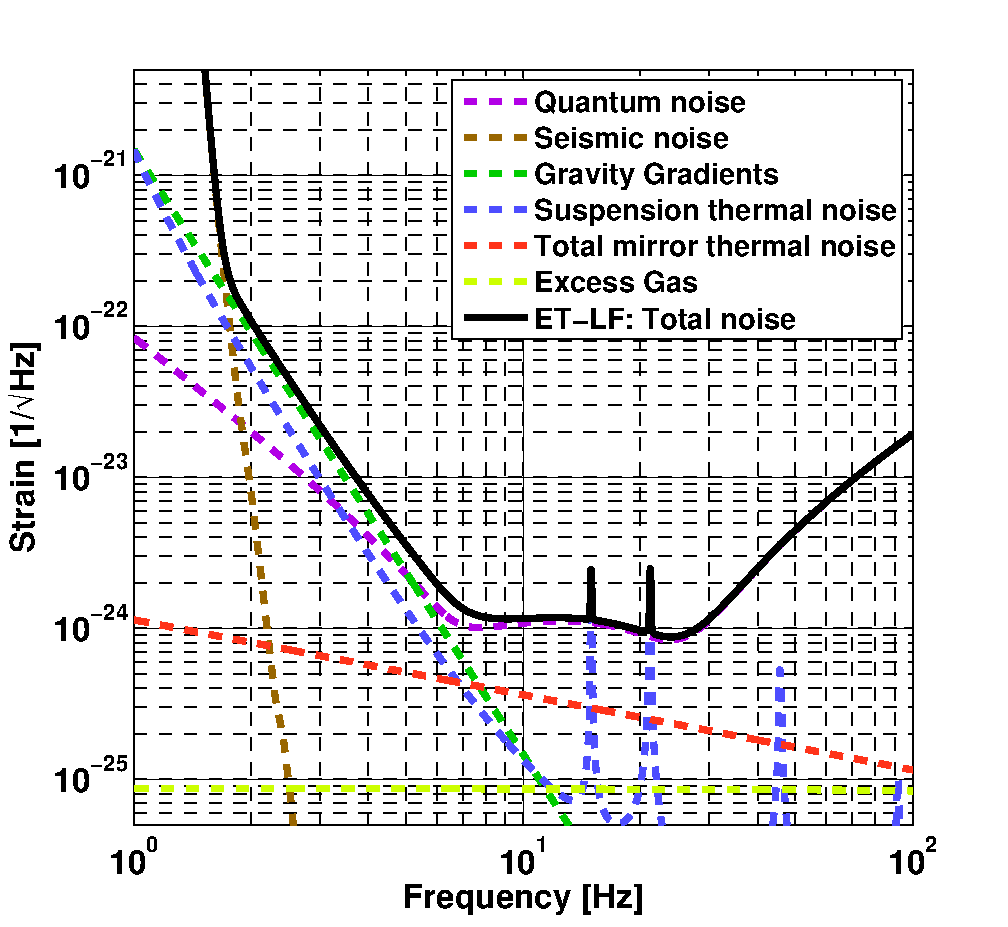
\includegraphics[width=0.45\textwidth]{Intro/Intro_Figures/ETD_LF3.pdf}
    \caption{Noise budget for the low- and high-frequency interferometer for the 
    parameters used for the ET-D sensitivity curve as stated in table~\ref{tab:summary14}.}
    \label{fig:noise_budget}
    \vspace{-0.7cm}
  \end{center}
\end{wrapfigure}

The xylophone strategy, i.e.\ the division of each detector into a low-frequency 
and a high-frequency interferometer, allows to pursue different strategies in 
optimising the noise for each frequency range. The noise budget for the 
high-frequency interferometer is shown in the upper part of figure~\ref{fig:noise_budget}. 

In the frequency range from about 7\,Hz to 30\,Hz the sensitivity is limited by
suspension thermal noise, resulting from the interferometer being operated 
at room temperature. At frequencies above 500\,Hz the dominating noise 
source is photon shot noise. Between these two frequency ranges mirror 
thermal noise is limiting the overall sensitivity. In the noise budget for the 
low-frequency interferometer, shown in the lower part of 
figure~\ref{fig:noise_budget}, quantum noise is limiting the sensitivity over 
the entire frequency range above 7\,Hz. Due to the operation at cryogenic 
temperatures the influence of suspension thermal noise in the frequency 
range above 7\,Hz can be cut down to a sufficiently low level. Below 7\,Hz 
the sensitivity is limited by comparable amounts of quantum noise, 
gravity gradient noise, and suspension thermal noise. Due to the good 
performance of the multistage pendulum suspensions the influence of 
seismic noise can be limited to the frequency range below 2\,Hz. Investigations 
of new quantum non-demolition techniques in a planned R\&D program will 
show whether it is possible to cut down the quantum noise contributions to 
an even lower level in the frequency range from 7\,Hz to 30\,Hz.

\FloatBarrier
\clearpage
\subsection{Layout of the observatory}
%\emph{Authors: M.Punturo, H. Lueck} \\

\begin{wrapfigure}{r}{0.6\textwidth}
\centering
\vskip -0.35cm
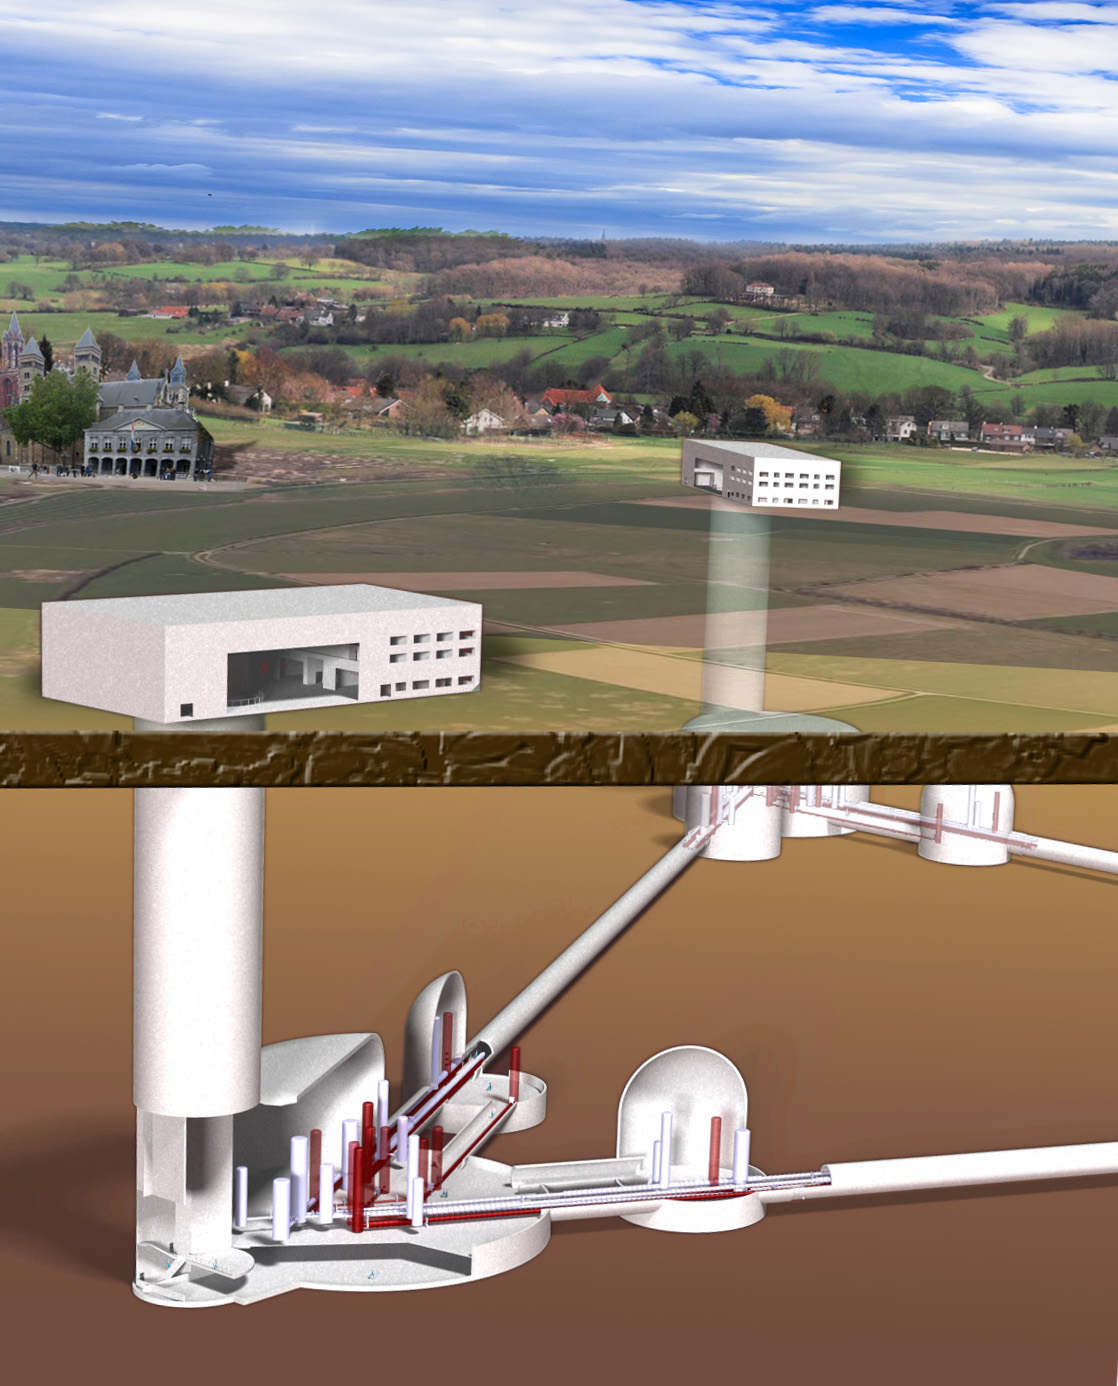
\includegraphics[width=0.6\textwidth]{Intro/Intro_Figures/ArtisticViewBuildings.jpg}
\vskip 0.3cm
\caption{Artistic view of the arrangement of buildings, access shafts and underground caverns.}
\vskip -0.1cm
\label{Fig:Buildings}
\end{wrapfigure} 

As a consequence of the extremely demanding seismic requirements the Einstein Telescope will be located underground at a depth of about 100\,m to 200\,m and will, in the complete configuration, consist of three nested detectors, each in turn composed of two interferometers. Selecting the geometry of an equilateral triangle,  where each side of the triangle is simultaneously used by two detector arms, allows to determine the polarisation of the gravitational wave and optimises the usage of the tunnels. The topology of each interferometer will be the dual-recycled Michelson layout with Fabry-Perot arm cavities. An artist's impression of the Einstein Telescope is shown in figure~\ref{fig:ET_artists_view}. \\
Underground seismic measurements at eight different European locations have been performed within this design study and additional measurements from external sources have also been evaluated. Satisfactory seismic performance has been found in several locations. 

For the final site selection long-term seismic noise measurements including seasonal effects like variable wind speeds and ocean wave height need to be made, and other nonscientific factors of influence (e.g.\ political, financial, interest of local parties, vicinity to research institutions) have to be included in the decision process.

The sensitivity curve shown in figure~\ref{fig:ET_sensitivity} gives the sensitivity for a single detector with 10\,km arm length and an angle of $90^{\circ}$ between the arms. This is done for better comparison with the existing detectors and their `advanced' versions. ET will in fact have three 10\,km detectors and the angles between the arms will be $60^{\circ}$. The resulting sensitivity in comparison with a single $90^{\circ}$ detector depends on the source location in the sky and its orientation, as the angular antenna pattern (see figure \ref{fig:triangleAP}) and the polarization dependence (independent in the triangular case) influence the signal strength differently for different detector layouts. On average the sensitivity of the triple $60^{\circ}$ detector is slightly better than a single, optimally oriented $90^{\circ}$ one.

\begin{tcolorbox}[standard jigsaw,colframe=green!40!black,colback=blanchedalmond!10!white,opacityback=0.6,coltext=black, title= {\bf Sensitivity curves for the Einstein Telescope}]
%\ETbox{h}{ETSensitivityCurves}{Sensitivity curves for the Einstein Telescope}
{As the understanding of the achievable sensitivity of the Einstein Telescope evolved  throughout the Design Study, different sensitivity curves are used in this document,  named from ET-B to ET-D (see figure~\ref{fig:ET_sens_evolution_2}).\\ 
The very first, preliminary sensitivity curve ET-A was a crude, early estimate and will hence not be used in this document. 
ET-B is the sensitivity curve where each detector is built from a single interferometer, where the high power needed to achieve good high-frequency performance compromises the low-frequency performance. Over a wide frequency range from a few Hertz to a few times 10\,Hz the sensitivity is limited by radiation pressure noise, whereas above a few hundred Hertz the sensitivity is limited by shot noise.\\
The next evolutionary step is the sensitivity curve ET-C, where each detector is split into two interferometers, each dedicated to a distinct frequency range (the xylophone configuration). Some technical details, such as losses inside optical resonators are not fully included in this sensitivity curve.\\
The latest sensitivity curve is given by ET-D, where imperfections like optical losses in cavities are included in the computations. As the later sensitivity curves 
became available only during the Design Study, some of the subsection results are still based on earlier versions, which will be indicated by the sensitivity curve acronym.\\
In the cost optimisation phase towards the end of the design study some parameters have been changed with respect to the ET-D sensitivity parameters, e.g.\ the lengths of the filter cavities for the high frequency interferometers, but have only an insignificant (<10\%) influence on the overall sensitivity.
\begin{figure}[H]
	\begin{center}
		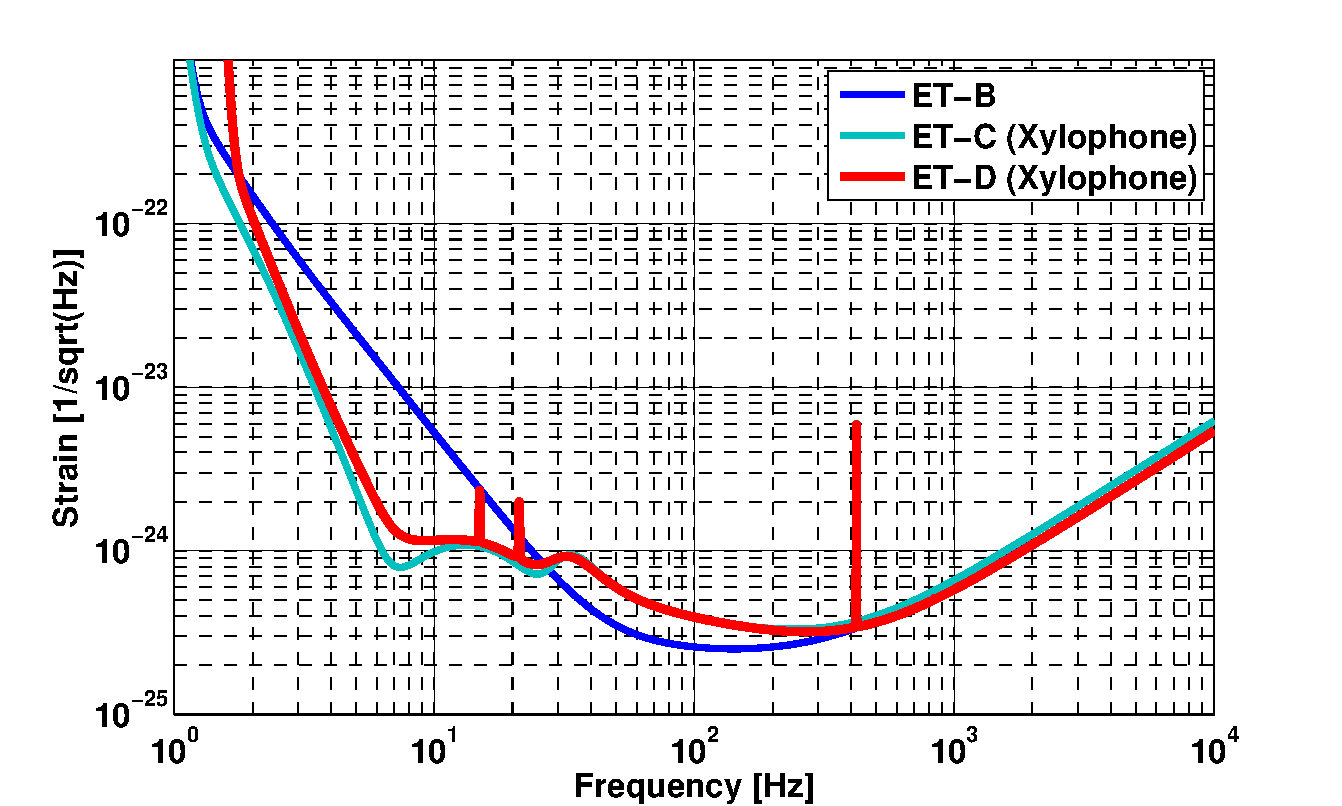
\includegraphics[width=0.7\textwidth]{Intro/Intro_Figures/all_sens3.pdf}
\vskip 0.3cm
	\caption{Sensitivity curves for ET used in this document. For details see text.}
	\label{fig:ET_sens_evolution_2}
	\end{center}
\vskip -0.4cm
\end{figure}
}
\end{tcolorbox}
For the desired sensitivity an overall side length of the triangle of about 10\,km is required. More specifically in this document we assume 10\,km for the arm cavity length as depicted in figure~\ref{fig:infra2} and figure \ref{Fig:Simple_ETv1} and an additional 300\,m of tunnel length for telescopes for mode matching the large beam size from the interferometer arms to smaller beams in the beam splitter area. 
This gives a total triangle side length of 10.3\,km and an overall tunnel length for the Einstein Telescope Observatory of 30.9\,km. This length of 300\,m from the ``vertex station'' to the ``satellite station'' is also used for the filter cavities for the high-frequency interferometer housed in a separate tunnel, which simultaneously serves as a safety escape route from the ``satellite caverns'' (see figure\,\ref{shaftaccess} and figure,\ref{infra}.  

\begin{wrapfigure}{r}{0.66\textwidth}
	\centering
\vskip 0.1cm
		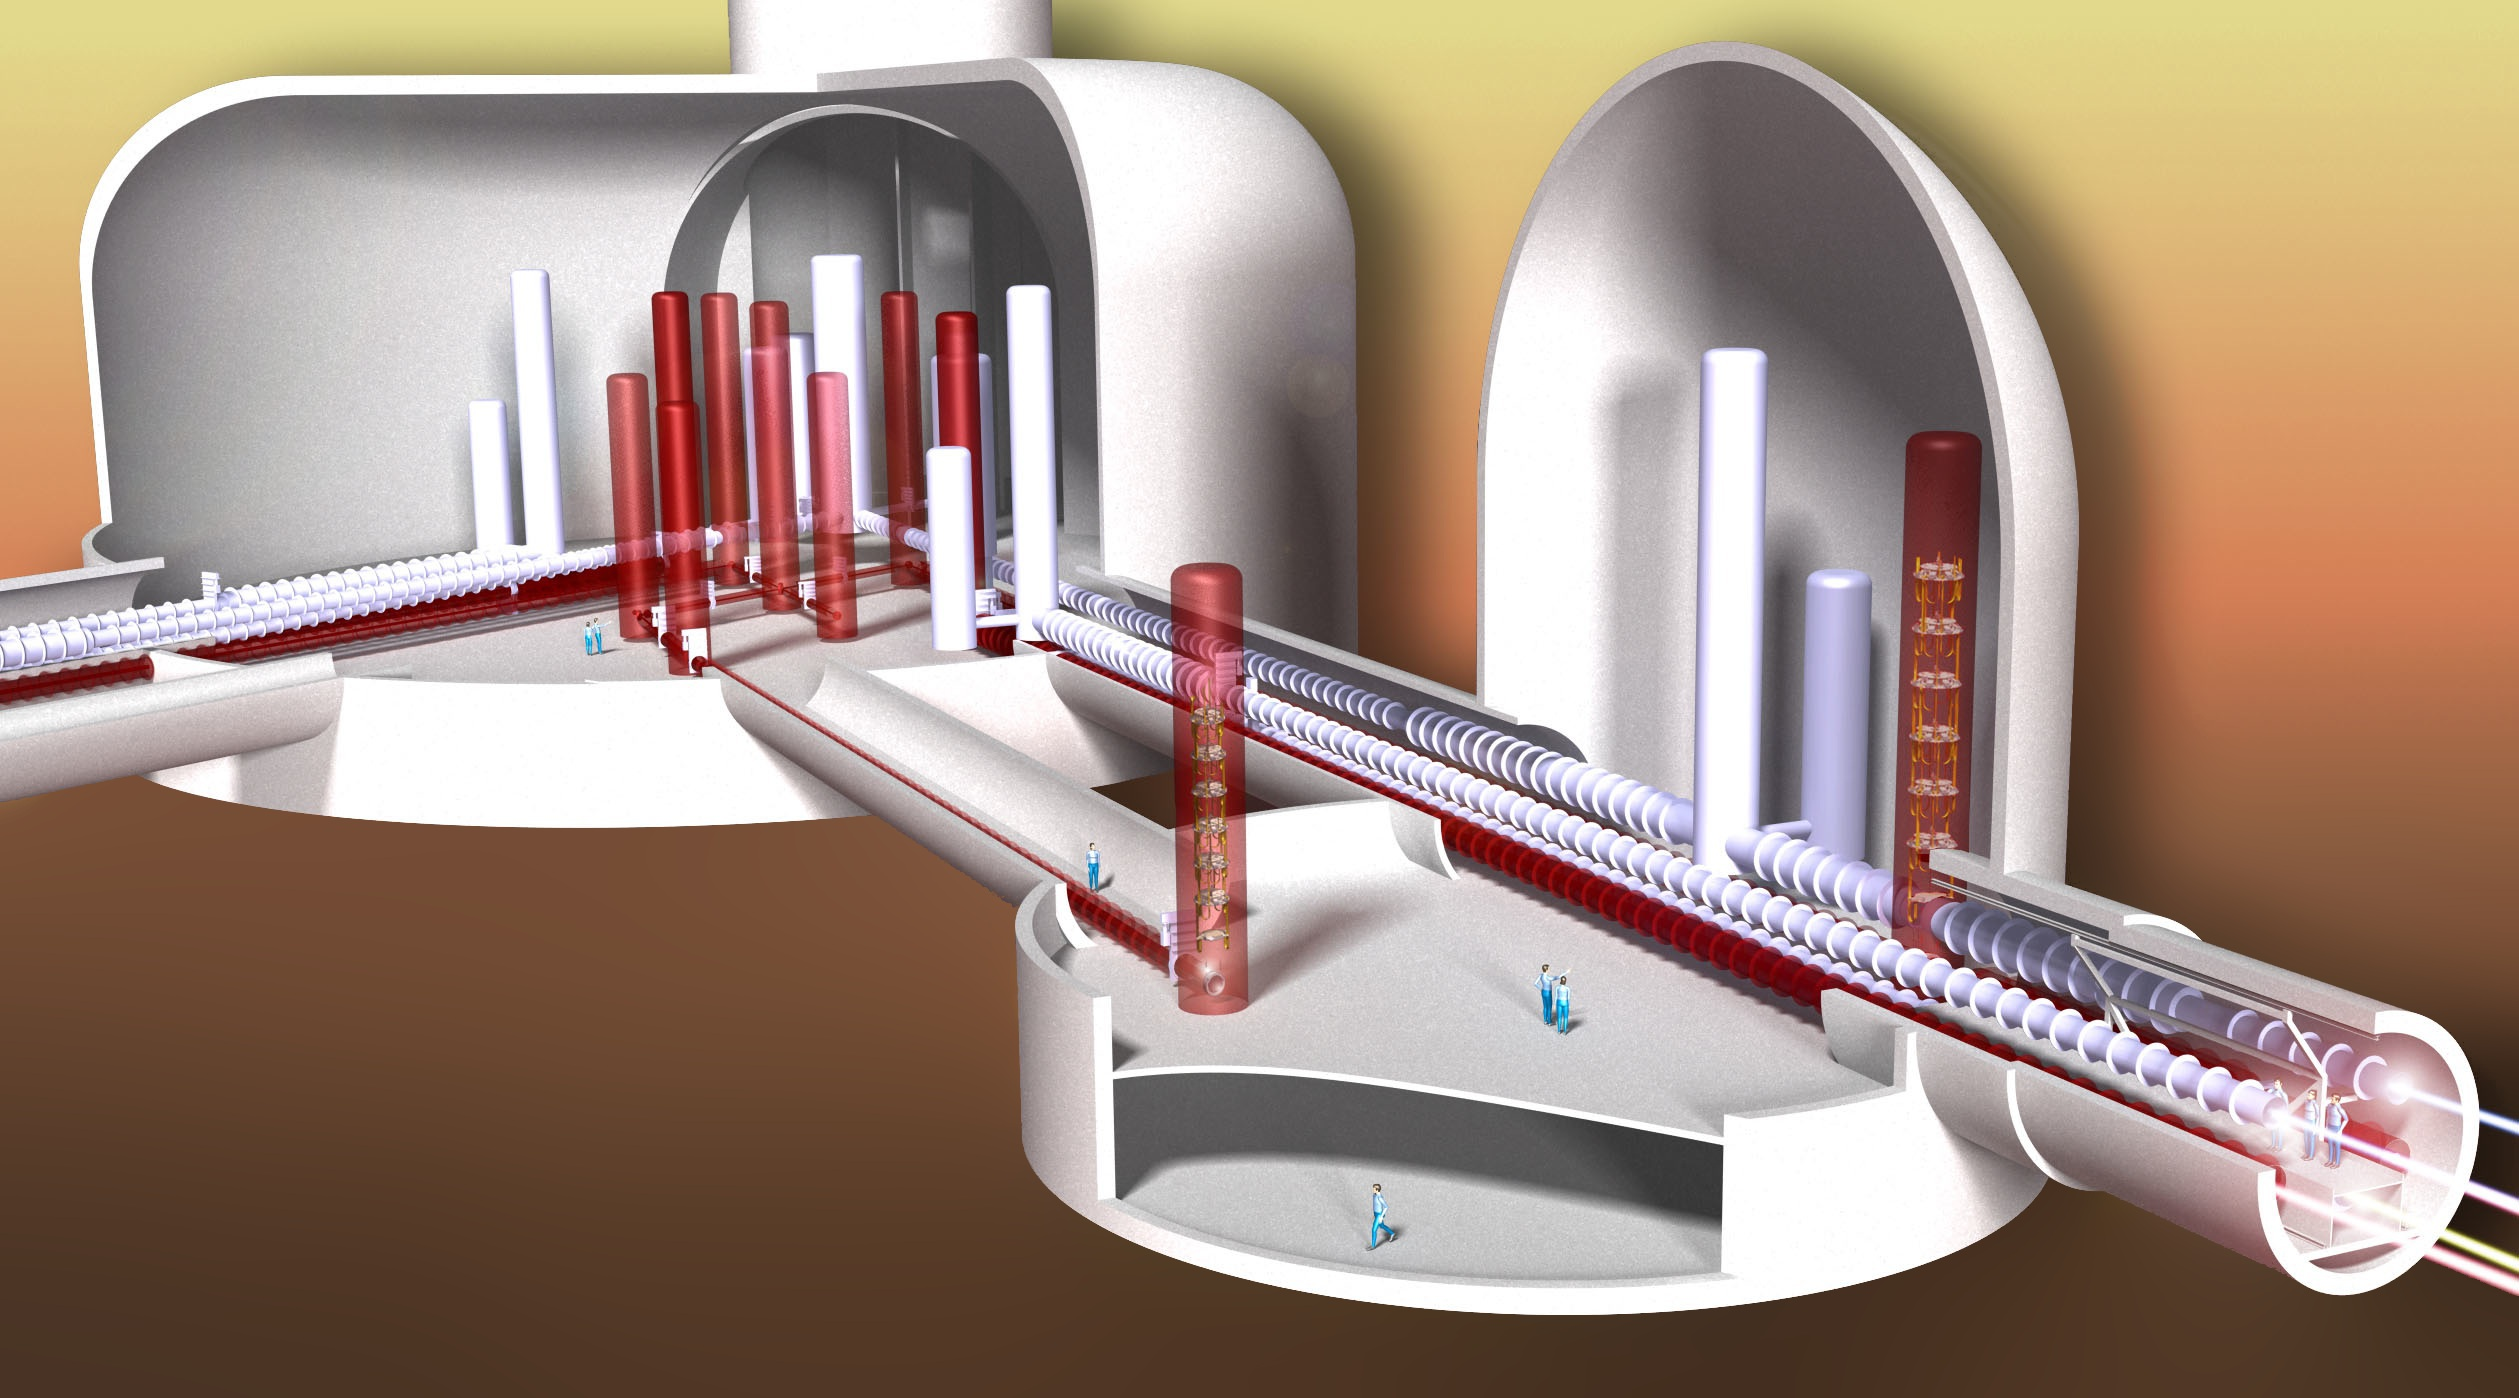
\includegraphics[width=0.66\textwidth]{Intro/Intro_Figures/ArtisticView1.jpg}
	\caption{Artistic impression of the underground arrangement of tunnels and 
	caverns. For details see sections~\ref{subsec:tunnels} and \ref{subsec:caverns}}
	\label{fig:Artisticview1}
\end{wrapfigure}
The main $\simeq$10\,km tunnels that \mbox{connect} two satellite stations (see section~\ref{subsec:tunnels}) will have an inner diameter of 5.5\,m, which will \mbox{locally} be increased to 6.0\,m wherever the insulation for \mbox{cryogenic} operation requires more space. The three {\mbox vertex} caverns and six satellite caverns will house the vacuum \mbox{vessels} and must be about 25\,m high (see section \ref{subsec:caverns}). 
Access to the \mbox{underground} detectors is foreseen via vertical shafts (see figure~\ref{fig:infra}). It remains to be explored in a technical design phase after site selection whether horizontal access is favourable. This option may, for instance, be advantageous if the \mbox{Observatory} is built inside a mountain. 

The ET infrastructure will house the observatory for many decades, during which the interferometers will receive upgrades as technology advances. Some of these changes may result in the necessity to change mirror positions and with it vacuum tank positions as we now see in the upgrades from the `initial' to the `advanced' generation of gravitational wave detectors. Hence we plan to build large caverns where the tanks can be placed at arbitrary positions, instead of building an inflexible system of short tunnels connecting narrow but tall caverns housing a single vacuum tank each.  

Above ground, at the entrance to the vertical axis shafts, facilities housing workshops, offices, apartments, technical facilities providing cryogenic fluids, air conditioning and venting, emergency electricity generators, etc.\ will be set up, as shown in figure \ref{fig:infra}. 
One major aspect of the design of the total infrastructure is to provide an environment able to house not only the basic initial version of the Einstein telescope that we describe in this Design Study document but also be versatile enough to accommodate upgraded versions in the following decades to come.   
\FloatBarrier
\subsection{Observatory timeline}
%\emph{Authors: M.Punturo, H. Lueck} \\
The realization of the ET observatory will be the final step of a long path and the initial act of a new scientific adventure. Several steps have been necessary (see Sec.~\ref{TimelineSubSection}) to allow the realization of this conceptual design study document  and few other important achievements are needed to reach the readiness condition for the observatory realization. The design of the new detector must evolve from the current conceptual phase to the technical design phase, successful R\&D activities must confirm the feasibility of the solutions proposed in this document, but, first of all, it is crucial that advanced detectors confirm the effectiveness of their new technologies and that a gravitational wave signal is detected in these interferometers. 
The detection of gravitational waves is regarded as a prerequisite for the start of construction of the Einstein Telescope.
For this reason the excavation of the ET site cannot start before 2017, and hence 2018 is here taken as the initial time ($t_0$) for the ET observatory realization. ET being an observatory that will be \emph{on line} for decades, priority in construction will be attributed to the site and infrastructures realization, selecting a modular philosophy for the detectors that will allow to implement the different interferometers composing each detector with a schedule stretched in time. In this way, after about 6 years of construction, installation and commissioning, the first detector of the ET observatory could be operative at the end of the first half of the next decade.
\FloatBarrier
\subsection{Observatory costs}
%\emph{Authors: M.Punturo, H. Lueck} \\
At this stage of the conceptual design the costs of the Observatory have to be regarded as a rough estimate. A summary of the estimated costs is shown in figure~\ref{Fig:TotalCostTable}. More details on the costing are explained in section~\ref{ConclusionsCostsSubSection}. 
The overall costs of an underground facility like the Einstein Telescope Observatory are dominated by excavation costs and construction of the underground tunnels and caverns. These costs depend significantly on the location and type of soil. In this design study a rather conservative assumption of260\,\texteuro$\rm{/m^3}$  has been made. The costs listed in the figure~\ref{Fig:TotalCostTable} assume a single detector to be implemented first. The costs include spares for each individual item. In most instances the spares will remain unused and can act as spares for the subsequent installation of the other two detectors, reducing their price tags somewhat.
